\documentclass[twoside]{book}

% Packages required by doxygen
\usepackage{fixltx2e}
\usepackage{calc}
\usepackage{doxygen}
\usepackage[export]{adjustbox} % also loads graphicx
\usepackage{graphicx}
\usepackage[utf8]{inputenc}
\usepackage{makeidx}
\usepackage{multicol}
\usepackage{multirow}
\PassOptionsToPackage{warn}{textcomp}
\usepackage{textcomp}
\usepackage[nointegrals]{wasysym}
\usepackage[table]{xcolor}

% Font selection
\usepackage[T1]{fontenc}
\usepackage[scaled=.90]{helvet}
\usepackage{courier}
\usepackage{amssymb}
\usepackage{sectsty}
\renewcommand{\familydefault}{\sfdefault}
\allsectionsfont{%
  \fontseries{bc}\selectfont%
  \color{darkgray}%
}
\renewcommand{\DoxyLabelFont}{%
  \fontseries{bc}\selectfont%
  \color{darkgray}%
}
\newcommand{\+}{\discretionary{\mbox{\scriptsize$\hookleftarrow$}}{}{}}

% Page & text layout
\usepackage{geometry}
\geometry{%
  a4paper,%
  top=2.5cm,%
  bottom=2.5cm,%
  left=2.5cm,%
  right=2.5cm%
}
\tolerance=750
\hfuzz=15pt
\hbadness=750
\setlength{\emergencystretch}{15pt}
\setlength{\parindent}{0cm}
\setlength{\parskip}{3ex plus 2ex minus 2ex}
\makeatletter
\renewcommand{\paragraph}{%
  \@startsection{paragraph}{4}{0ex}{-1.0ex}{1.0ex}{%
    \normalfont\normalsize\bfseries\SS@parafont%
  }%
}
\renewcommand{\subparagraph}{%
  \@startsection{subparagraph}{5}{0ex}{-1.0ex}{1.0ex}{%
    \normalfont\normalsize\bfseries\SS@subparafont%
  }%
}
\makeatother

% Headers & footers
\usepackage{fancyhdr}
\pagestyle{fancyplain}
\fancyhead[LE]{\fancyplain{}{\bfseries\thepage}}
\fancyhead[CE]{\fancyplain{}{}}
\fancyhead[RE]{\fancyplain{}{\bfseries\leftmark}}
\fancyhead[LO]{\fancyplain{}{\bfseries\rightmark}}
\fancyhead[CO]{\fancyplain{}{}}
\fancyhead[RO]{\fancyplain{}{\bfseries\thepage}}
\fancyfoot[LE]{\fancyplain{}{}}
\fancyfoot[CE]{\fancyplain{}{}}
\fancyfoot[RE]{\fancyplain{}{\bfseries\scriptsize Generated by Doxygen }}
\fancyfoot[LO]{\fancyplain{}{\bfseries\scriptsize Generated by Doxygen }}
\fancyfoot[CO]{\fancyplain{}{}}
\fancyfoot[RO]{\fancyplain{}{}}
\renewcommand{\footrulewidth}{0.4pt}
\renewcommand{\chaptermark}[1]{%
  \markboth{#1}{}%
}
\renewcommand{\sectionmark}[1]{%
  \markright{\thesection\ #1}%
}

% Indices & bibliography
\usepackage{natbib}
\usepackage[titles]{tocloft}
\setcounter{tocdepth}{3}
\setcounter{secnumdepth}{5}
\makeindex

% Hyperlinks (required, but should be loaded last)
\usepackage{ifpdf}
\ifpdf
  \usepackage[pdftex,pagebackref=true]{hyperref}
\else
  \usepackage[ps2pdf,pagebackref=true]{hyperref}
\fi
\hypersetup{%
  colorlinks=true,%
  linkcolor=blue,%
  citecolor=blue,%
  unicode%
}

% Custom commands
\newcommand{\clearemptydoublepage}{%
  \newpage{\pagestyle{empty}\cleardoublepage}%
}

\usepackage{caption}
\captionsetup{labelsep=space,justification=centering,font={bf},singlelinecheck=off,skip=4pt,position=top}

%===== C O N T E N T S =====

\begin{document}

% Titlepage & ToC
\hypersetup{pageanchor=false,
             bookmarksnumbered=true,
             pdfencoding=unicode
            }
\pagenumbering{roman}
\begin{titlepage}
\vspace*{7cm}
\begin{center}%
{\Large My Project }\\
\vspace*{1cm}
{\large Generated by Doxygen 1.8.11}\\
\end{center}
\end{titlepage}
\clearemptydoublepage
\tableofcontents
\clearemptydoublepage
\pagenumbering{arabic}
\hypersetup{pageanchor=true}

%--- Begin generated contents ---
\chapter{File Index}
\section{File List}
Here is a list of all files with brief descriptions\+:\begin{DoxyCompactList}
\item\contentsline{section}{\hyperlink{Lab1_8c}{Lab1.\+c} }{\pageref{Lab1_8c}}{}
\end{DoxyCompactList}

\chapter{File Documentation}
\hypertarget{RSA_8cpp}{}\section{R\+S\+A.\+cpp File Reference}
\label{RSA_8cpp}\index{R\+S\+A.\+cpp@{R\+S\+A.\+cpp}}
{\ttfamily \#include $<$iostream$>$}\\*
{\ttfamily \#include $<$math.\+h$>$}\\*
{\ttfamily \#include $<$string.\+h$>$}\\*
{\ttfamily \#include $<$stdlib.\+h$>$}\\*
Include dependency graph for R\+S\+A.\+cpp\+:
\nopagebreak
\begin{figure}[H]
\begin{center}
\leavevmode
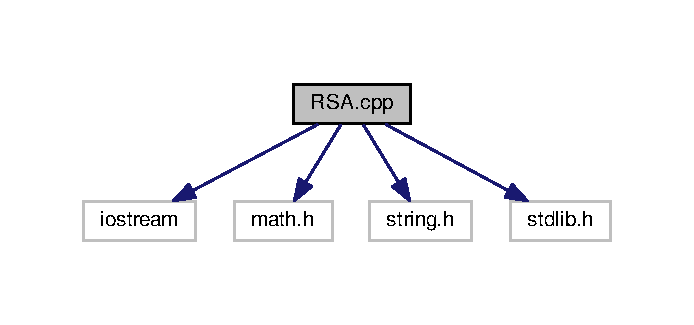
\includegraphics[width=333pt]{RSA_8cpp__incl}
\end{center}
\end{figure}
\subsection*{Functions}
\begin{DoxyCompactItemize}
\item 
int \hyperlink{RSA_8cpp_af6b44243040407da87e2598a39616ef9}{prime} (long int)
\item 
void \hyperlink{RSA_8cpp_a6cad623c3a6b97ae93c176910f6ec51b}{ce} ()
\item 
long int \hyperlink{RSA_8cpp_a09cf6985f716e8441d9510bb4d9666dd}{cd} (long int)
\item 
void \hyperlink{RSA_8cpp_a69d798b95510d739e99e0e78ea464660}{encrypt} ()
\item 
void \hyperlink{RSA_8cpp_a4926a93501a38e100d0ff8bc82259527}{decrypt} ()
\item 
int \hyperlink{RSA_8cpp_ae66f6b31b5ad750f1fe042a706a4e3d4}{main} ()
\end{DoxyCompactItemize}
\subsection*{Variables}
\begin{DoxyCompactItemize}
\item 
long int \hyperlink{RSA_8cpp_acd6f73fb1a6f78a968560d6ec881eb58}{p}
\item 
long int \hyperlink{RSA_8cpp_a2bf403c7ef4a7e7f626ade25b718c2bd}{q}
\item 
long int \hyperlink{RSA_8cpp_a35c5d787326025a70aa82d22dabe6305}{n}
\item 
long int \hyperlink{RSA_8cpp_a8e25edb779baee2272328042ced15002}{t}
\item 
long int \hyperlink{RSA_8cpp_a25bed4d6600e3d6d5e7dae21ccaa899f}{flag}
\item 
long int \hyperlink{RSA_8cpp_a2c3bcb43f977cc3d1b3a89a0a048bc2a}{e} \mbox{[}100\mbox{]}
\item 
long int \hyperlink{RSA_8cpp_ac23e2a55ef75166c8d32f5d995ca5c02}{d} \mbox{[}100\mbox{]}
\item 
long int \hyperlink{RSA_8cpp_a52cd0abaa4e7404902e64b06db7257c6}{temp} \mbox{[}100\mbox{]}
\item 
long int \hyperlink{RSA_8cpp_aaf120c998f82e99546e2ac0f7491f227}{j}
\item 
long int \hyperlink{RSA_8cpp_a50c9f88f172b8f98f1a5848e4ceb9932}{m} \mbox{[}100\mbox{]}
\item 
long int \hyperlink{RSA_8cpp_ab422116306fa250a781fd1929dbf08a7}{en} \mbox{[}100\mbox{]}
\item 
long int \hyperlink{RSA_8cpp_ac1e8399c83da2b276b2200593325411f}{i}
\item 
char \hyperlink{RSA_8cpp_a184b5dd9844bf6e022deb71044ff7f64}{msg} \mbox{[}100\mbox{]}
\end{DoxyCompactItemize}


\subsection{Function Documentation}
\index{R\+S\+A.\+cpp@{R\+S\+A.\+cpp}!cd@{cd}}
\index{cd@{cd}!R\+S\+A.\+cpp@{R\+S\+A.\+cpp}}
\subsubsection[{\texorpdfstring{cd(long int)}{cd(long int)}}]{\setlength{\rightskip}{0pt plus 5cm}long int cd (
\begin{DoxyParamCaption}
\item[{long int}]{x}
\end{DoxyParamCaption}
)}\hypertarget{RSA_8cpp_a09cf6985f716e8441d9510bb4d9666dd}{}\label{RSA_8cpp_a09cf6985f716e8441d9510bb4d9666dd}

\begin{DoxyCode}
86 \{
87     \textcolor{keywordtype}{long} \textcolor{keywordtype}{int} k = 1;
88     \textcolor{keywordflow}{while} (1)
89     \{
90         k = k + \hyperlink{RSA_8cpp_a8e25edb779baee2272328042ced15002}{t};
91         \textcolor{keywordflow}{if} (k % x == 0)
92             \textcolor{keywordflow}{return} (k / x);
93     \}
94 \}
\end{DoxyCode}
\index{R\+S\+A.\+cpp@{R\+S\+A.\+cpp}!ce@{ce}}
\index{ce@{ce}!R\+S\+A.\+cpp@{R\+S\+A.\+cpp}}
\subsubsection[{\texorpdfstring{ce()}{ce()}}]{\setlength{\rightskip}{0pt plus 5cm}void ce (
\begin{DoxyParamCaption}
{}
\end{DoxyParamCaption}
)}\hypertarget{RSA_8cpp_a6cad623c3a6b97ae93c176910f6ec51b}{}\label{RSA_8cpp_a6cad623c3a6b97ae93c176910f6ec51b}

\begin{DoxyCode}
63 \{
64     \textcolor{keywordtype}{int} k;
65     k = 0;
66     \textcolor{keywordflow}{for} (\hyperlink{RSA_8cpp_ac1e8399c83da2b276b2200593325411f}{i} = 2; \hyperlink{RSA_8cpp_ac1e8399c83da2b276b2200593325411f}{i} < \hyperlink{RSA_8cpp_a8e25edb779baee2272328042ced15002}{t}; \hyperlink{RSA_8cpp_ac1e8399c83da2b276b2200593325411f}{i}++)
67     \{
68         \textcolor{keywordflow}{if} (t % \hyperlink{RSA_8cpp_ac1e8399c83da2b276b2200593325411f}{i} == 0)
69             \textcolor{keywordflow}{continue};
70         \hyperlink{RSA_8cpp_a25bed4d6600e3d6d5e7dae21ccaa899f}{flag} = \hyperlink{RSA_8cpp_af6b44243040407da87e2598a39616ef9}{prime}(\hyperlink{RSA_8cpp_ac1e8399c83da2b276b2200593325411f}{i});
71         \textcolor{keywordflow}{if} (\hyperlink{RSA_8cpp_a25bed4d6600e3d6d5e7dae21ccaa899f}{flag} == 1 && \hyperlink{RSA_8cpp_ac1e8399c83da2b276b2200593325411f}{i} != \hyperlink{RSA_8cpp_acd6f73fb1a6f78a968560d6ec881eb58}{p} && \hyperlink{RSA_8cpp_ac1e8399c83da2b276b2200593325411f}{i} != \hyperlink{RSA_8cpp_a2bf403c7ef4a7e7f626ade25b718c2bd}{q})
72         \{
73             \hyperlink{RSA_8cpp_a2c3bcb43f977cc3d1b3a89a0a048bc2a}{e}[k] = \hyperlink{RSA_8cpp_ac1e8399c83da2b276b2200593325411f}{i};
74             \hyperlink{RSA_8cpp_a25bed4d6600e3d6d5e7dae21ccaa899f}{flag} = \hyperlink{RSA_8cpp_a09cf6985f716e8441d9510bb4d9666dd}{cd}(\hyperlink{RSA_8cpp_a2c3bcb43f977cc3d1b3a89a0a048bc2a}{e}[k]);
75             \textcolor{keywordflow}{if} (\hyperlink{RSA_8cpp_a25bed4d6600e3d6d5e7dae21ccaa899f}{flag} > 0)
76             \{
77                 \hyperlink{RSA_8cpp_ac23e2a55ef75166c8d32f5d995ca5c02}{d}[k] = \hyperlink{RSA_8cpp_a25bed4d6600e3d6d5e7dae21ccaa899f}{flag};
78                 k++;
79             \}
80             \textcolor{keywordflow}{if} (k == 99)
81                 \textcolor{keywordflow}{break};
82         \}
83     \}
84 \}
\end{DoxyCode}


Here is the call graph for this function\+:
\nopagebreak
\begin{figure}[H]
\begin{center}
\leavevmode
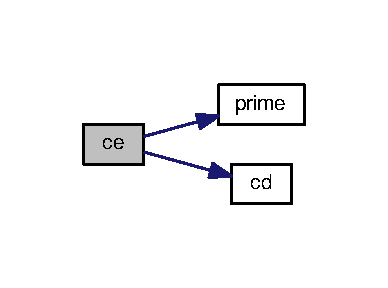
\includegraphics[width=186pt]{RSA_8cpp_a6cad623c3a6b97ae93c176910f6ec51b_cgraph}
\end{center}
\end{figure}


\index{R\+S\+A.\+cpp@{R\+S\+A.\+cpp}!decrypt@{decrypt}}
\index{decrypt@{decrypt}!R\+S\+A.\+cpp@{R\+S\+A.\+cpp}}
\subsubsection[{\texorpdfstring{decrypt()}{decrypt()}}]{\setlength{\rightskip}{0pt plus 5cm}void decrypt (
\begin{DoxyParamCaption}
{}
\end{DoxyParamCaption}
)}\hypertarget{RSA_8cpp_a4926a93501a38e100d0ff8bc82259527}{}\label{RSA_8cpp_a4926a93501a38e100d0ff8bc82259527}

\begin{DoxyCode}
121 \{
122     \textcolor{keywordtype}{long} \textcolor{keywordtype}{int} pt, ct, key = \hyperlink{RSA_8cpp_ac23e2a55ef75166c8d32f5d995ca5c02}{d}[0], k;
123     \hyperlink{RSA_8cpp_ac1e8399c83da2b276b2200593325411f}{i} = 0;
124     \textcolor{keywordflow}{while} (\hyperlink{RSA_8cpp_ab422116306fa250a781fd1929dbf08a7}{en}[\hyperlink{RSA_8cpp_ac1e8399c83da2b276b2200593325411f}{i}] != -1)
125     \{
126         ct = \hyperlink{RSA_8cpp_a52cd0abaa4e7404902e64b06db7257c6}{temp}[\hyperlink{RSA_8cpp_ac1e8399c83da2b276b2200593325411f}{i}];
127         k = 1;
128         \textcolor{keywordflow}{for} (\hyperlink{RSA_8cpp_aaf120c998f82e99546e2ac0f7491f227}{j} = 0; \hyperlink{RSA_8cpp_aaf120c998f82e99546e2ac0f7491f227}{j} < key; \hyperlink{RSA_8cpp_aaf120c998f82e99546e2ac0f7491f227}{j}++)
129         \{
130             k = k * ct;
131             k = k % \hyperlink{RSA_8cpp_a35c5d787326025a70aa82d22dabe6305}{n};
132         \}
133         pt = k + 96;
134         \hyperlink{RSA_8cpp_a50c9f88f172b8f98f1a5848e4ceb9932}{m}[\hyperlink{RSA_8cpp_ac1e8399c83da2b276b2200593325411f}{i}] = pt;
135         \hyperlink{RSA_8cpp_ac1e8399c83da2b276b2200593325411f}{i}++;
136     \}
137     \hyperlink{RSA_8cpp_a50c9f88f172b8f98f1a5848e4ceb9932}{m}[\hyperlink{RSA_8cpp_ac1e8399c83da2b276b2200593325411f}{i}] = -1;
138     cout << \textcolor{stringliteral}{"\(\backslash\)nTHE DECRYPTED MESSAGE IS\(\backslash\)n"};
139     \textcolor{keywordflow}{for} (\hyperlink{RSA_8cpp_ac1e8399c83da2b276b2200593325411f}{i} = 0; \hyperlink{RSA_8cpp_a50c9f88f172b8f98f1a5848e4ceb9932}{m}[\hyperlink{RSA_8cpp_ac1e8399c83da2b276b2200593325411f}{i}] != -1; \hyperlink{RSA_8cpp_ac1e8399c83da2b276b2200593325411f}{i}++)
140         printf(\textcolor{stringliteral}{"%c"}, \hyperlink{RSA_8cpp_a50c9f88f172b8f98f1a5848e4ceb9932}{m}[\hyperlink{RSA_8cpp_ac1e8399c83da2b276b2200593325411f}{i}]);
141 \}
\end{DoxyCode}
\index{R\+S\+A.\+cpp@{R\+S\+A.\+cpp}!encrypt@{encrypt}}
\index{encrypt@{encrypt}!R\+S\+A.\+cpp@{R\+S\+A.\+cpp}}
\subsubsection[{\texorpdfstring{encrypt()}{encrypt()}}]{\setlength{\rightskip}{0pt plus 5cm}void encrypt (
\begin{DoxyParamCaption}
{}
\end{DoxyParamCaption}
)}\hypertarget{RSA_8cpp_a69d798b95510d739e99e0e78ea464660}{}\label{RSA_8cpp_a69d798b95510d739e99e0e78ea464660}

\begin{DoxyCode}
96 \{
97     \textcolor{keywordtype}{long} \textcolor{keywordtype}{int} pt, ct, key = \hyperlink{RSA_8cpp_a2c3bcb43f977cc3d1b3a89a0a048bc2a}{e}[0], k, len;
98     \hyperlink{RSA_8cpp_ac1e8399c83da2b276b2200593325411f}{i} = 0;
99     len = strlen(\hyperlink{RSA_8cpp_a184b5dd9844bf6e022deb71044ff7f64}{msg});
100     \textcolor{keywordflow}{while} (\hyperlink{RSA_8cpp_ac1e8399c83da2b276b2200593325411f}{i} != len)
101     \{
102         pt = \hyperlink{RSA_8cpp_a50c9f88f172b8f98f1a5848e4ceb9932}{m}[\hyperlink{RSA_8cpp_ac1e8399c83da2b276b2200593325411f}{i}];
103         pt = pt - 96;
104         k = 1;
105         \textcolor{keywordflow}{for} (\hyperlink{RSA_8cpp_aaf120c998f82e99546e2ac0f7491f227}{j} = 0; \hyperlink{RSA_8cpp_aaf120c998f82e99546e2ac0f7491f227}{j} < key; \hyperlink{RSA_8cpp_aaf120c998f82e99546e2ac0f7491f227}{j}++)
106         \{
107             k = k * pt;
108             k = k % \hyperlink{RSA_8cpp_a35c5d787326025a70aa82d22dabe6305}{n};
109         \}
110         \hyperlink{RSA_8cpp_a52cd0abaa4e7404902e64b06db7257c6}{temp}[\hyperlink{RSA_8cpp_ac1e8399c83da2b276b2200593325411f}{i}] = k;
111         ct = k + 96;
112         \hyperlink{RSA_8cpp_ab422116306fa250a781fd1929dbf08a7}{en}[\hyperlink{RSA_8cpp_ac1e8399c83da2b276b2200593325411f}{i}] = ct;
113         \hyperlink{RSA_8cpp_ac1e8399c83da2b276b2200593325411f}{i}++;
114     \}
115     \hyperlink{RSA_8cpp_ab422116306fa250a781fd1929dbf08a7}{en}[\hyperlink{RSA_8cpp_ac1e8399c83da2b276b2200593325411f}{i}] = -1;
116     cout << \textcolor{stringliteral}{"\(\backslash\)nTHE ENCRYPTED MESSAGE IS\(\backslash\)n"};
117     \textcolor{keywordflow}{for} (\hyperlink{RSA_8cpp_ac1e8399c83da2b276b2200593325411f}{i} = 0; \hyperlink{RSA_8cpp_ab422116306fa250a781fd1929dbf08a7}{en}[\hyperlink{RSA_8cpp_ac1e8399c83da2b276b2200593325411f}{i}] != -1; \hyperlink{RSA_8cpp_ac1e8399c83da2b276b2200593325411f}{i}++)
118         printf(\textcolor{stringliteral}{"%c"}, \hyperlink{RSA_8cpp_ab422116306fa250a781fd1929dbf08a7}{en}[\hyperlink{RSA_8cpp_ac1e8399c83da2b276b2200593325411f}{i}]);
119 \}
\end{DoxyCode}
\index{R\+S\+A.\+cpp@{R\+S\+A.\+cpp}!main@{main}}
\index{main@{main}!R\+S\+A.\+cpp@{R\+S\+A.\+cpp}}
\subsubsection[{\texorpdfstring{main()}{main()}}]{\setlength{\rightskip}{0pt plus 5cm}int main (
\begin{DoxyParamCaption}
{}
\end{DoxyParamCaption}
)}\hypertarget{RSA_8cpp_ae66f6b31b5ad750f1fe042a706a4e3d4}{}\label{RSA_8cpp_ae66f6b31b5ad750f1fe042a706a4e3d4}

\begin{DoxyCode}
30 \{
31     cout << \textcolor{stringliteral}{"\(\backslash\)nENTER FIRST PRIME NUMBER\(\backslash\)n"};
32     cin >> \hyperlink{RSA_8cpp_acd6f73fb1a6f78a968560d6ec881eb58}{p};
33     \hyperlink{RSA_8cpp_a25bed4d6600e3d6d5e7dae21ccaa899f}{flag} = \hyperlink{RSA_8cpp_af6b44243040407da87e2598a39616ef9}{prime}(p);
34     \textcolor{keywordflow}{if} (\hyperlink{RSA_8cpp_a25bed4d6600e3d6d5e7dae21ccaa899f}{flag} == 0)
35     \{
36         cout << \textcolor{stringliteral}{"\(\backslash\)nWRONG INPUT\(\backslash\)n"};
37         exit(1);
38     \}
39     cout << \textcolor{stringliteral}{"\(\backslash\)nENTER ANOTHER PRIME NUMBER\(\backslash\)n"};
40     cin >> \hyperlink{RSA_8cpp_a2bf403c7ef4a7e7f626ade25b718c2bd}{q};
41     \hyperlink{RSA_8cpp_a25bed4d6600e3d6d5e7dae21ccaa899f}{flag} = \hyperlink{RSA_8cpp_af6b44243040407da87e2598a39616ef9}{prime}(q);
42     \textcolor{keywordflow}{if} (\hyperlink{RSA_8cpp_a25bed4d6600e3d6d5e7dae21ccaa899f}{flag} == 0 || p == q)
43     \{
44         cout << \textcolor{stringliteral}{"\(\backslash\)nWRONG INPUT\(\backslash\)n"};
45         exit(1);
46     \}
47     cout << \textcolor{stringliteral}{"\(\backslash\)nENTER MESSAGE\(\backslash\)n"};
48     fflush(stdin);
49     cin >> \hyperlink{RSA_8cpp_a184b5dd9844bf6e022deb71044ff7f64}{msg};
50     \textcolor{keywordflow}{for} (\hyperlink{RSA_8cpp_ac1e8399c83da2b276b2200593325411f}{i} = 0; msg[\hyperlink{RSA_8cpp_ac1e8399c83da2b276b2200593325411f}{i}] != \textcolor{charliteral}{'\(\backslash\)0'}; \hyperlink{RSA_8cpp_ac1e8399c83da2b276b2200593325411f}{i}++)
51         \hyperlink{RSA_8cpp_a50c9f88f172b8f98f1a5848e4ceb9932}{m}[\hyperlink{RSA_8cpp_ac1e8399c83da2b276b2200593325411f}{i}] = msg[\hyperlink{RSA_8cpp_ac1e8399c83da2b276b2200593325411f}{i}];
52     \hyperlink{RSA_8cpp_a35c5d787326025a70aa82d22dabe6305}{n} = p * \hyperlink{RSA_8cpp_a2bf403c7ef4a7e7f626ade25b718c2bd}{q};
53     \hyperlink{RSA_8cpp_a8e25edb779baee2272328042ced15002}{t} = (p - 1) * (q - 1);
54     \hyperlink{RSA_8cpp_a6cad623c3a6b97ae93c176910f6ec51b}{ce}();
55     cout << \textcolor{stringliteral}{"\(\backslash\)nPOSSIBLE VALUES OF e AND d ARE\(\backslash\)n"};
56     \textcolor{keywordflow}{for} (\hyperlink{RSA_8cpp_ac1e8399c83da2b276b2200593325411f}{i} = 0; \hyperlink{RSA_8cpp_ac1e8399c83da2b276b2200593325411f}{i} < \hyperlink{RSA_8cpp_aaf120c998f82e99546e2ac0f7491f227}{j} - 1; \hyperlink{RSA_8cpp_ac1e8399c83da2b276b2200593325411f}{i}++)
57         cout << \hyperlink{RSA_8cpp_a2c3bcb43f977cc3d1b3a89a0a048bc2a}{e}[\hyperlink{RSA_8cpp_ac1e8399c83da2b276b2200593325411f}{i}] << \textcolor{stringliteral}{"\(\backslash\)t"} << \hyperlink{RSA_8cpp_ac23e2a55ef75166c8d32f5d995ca5c02}{d}[\hyperlink{RSA_8cpp_ac1e8399c83da2b276b2200593325411f}{i}] << \textcolor{stringliteral}{"\(\backslash\)n"};
58     \hyperlink{RSA_8cpp_a69d798b95510d739e99e0e78ea464660}{encrypt}();
59     \hyperlink{RSA_8cpp_a4926a93501a38e100d0ff8bc82259527}{decrypt}();
60     \textcolor{keywordflow}{return} 0;
61 \}
\end{DoxyCode}


Here is the call graph for this function\+:
\nopagebreak
\begin{figure}[H]
\begin{center}
\leavevmode
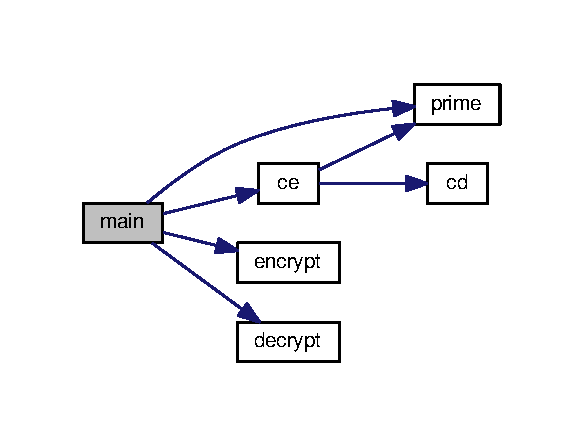
\includegraphics[width=280pt]{RSA_8cpp_ae66f6b31b5ad750f1fe042a706a4e3d4_cgraph}
\end{center}
\end{figure}


\index{R\+S\+A.\+cpp@{R\+S\+A.\+cpp}!prime@{prime}}
\index{prime@{prime}!R\+S\+A.\+cpp@{R\+S\+A.\+cpp}}
\subsubsection[{\texorpdfstring{prime(long int)}{prime(long int)}}]{\setlength{\rightskip}{0pt plus 5cm}int prime (
\begin{DoxyParamCaption}
\item[{long int}]{pr}
\end{DoxyParamCaption}
)}\hypertarget{RSA_8cpp_af6b44243040407da87e2598a39616ef9}{}\label{RSA_8cpp_af6b44243040407da87e2598a39616ef9}

\begin{DoxyCode}
19 \{
20     \textcolor{keywordtype}{int} \hyperlink{RSA_8cpp_ac1e8399c83da2b276b2200593325411f}{i};
21     \hyperlink{RSA_8cpp_aaf120c998f82e99546e2ac0f7491f227}{j} = sqrt(pr);
22     \textcolor{keywordflow}{for} (i = 2; i <= \hyperlink{RSA_8cpp_aaf120c998f82e99546e2ac0f7491f227}{j}; i++)
23     \{
24         \textcolor{keywordflow}{if} (pr % i == 0)
25             \textcolor{keywordflow}{return} 0;
26     \}
27     \textcolor{keywordflow}{return} 1;
28 \}
\end{DoxyCode}


\subsection{Variable Documentation}
\index{R\+S\+A.\+cpp@{R\+S\+A.\+cpp}!d@{d}}
\index{d@{d}!R\+S\+A.\+cpp@{R\+S\+A.\+cpp}}
\subsubsection[{\texorpdfstring{d}{d}}]{\setlength{\rightskip}{0pt plus 5cm}long int d\mbox{[}100\mbox{]}}\hypertarget{RSA_8cpp_ac23e2a55ef75166c8d32f5d995ca5c02}{}\label{RSA_8cpp_ac23e2a55ef75166c8d32f5d995ca5c02}
\index{R\+S\+A.\+cpp@{R\+S\+A.\+cpp}!e@{e}}
\index{e@{e}!R\+S\+A.\+cpp@{R\+S\+A.\+cpp}}
\subsubsection[{\texorpdfstring{e}{e}}]{\setlength{\rightskip}{0pt plus 5cm}long int e\mbox{[}100\mbox{]}}\hypertarget{RSA_8cpp_a2c3bcb43f977cc3d1b3a89a0a048bc2a}{}\label{RSA_8cpp_a2c3bcb43f977cc3d1b3a89a0a048bc2a}
\index{R\+S\+A.\+cpp@{R\+S\+A.\+cpp}!en@{en}}
\index{en@{en}!R\+S\+A.\+cpp@{R\+S\+A.\+cpp}}
\subsubsection[{\texorpdfstring{en}{en}}]{\setlength{\rightskip}{0pt plus 5cm}long int en\mbox{[}100\mbox{]}}\hypertarget{RSA_8cpp_ab422116306fa250a781fd1929dbf08a7}{}\label{RSA_8cpp_ab422116306fa250a781fd1929dbf08a7}
\index{R\+S\+A.\+cpp@{R\+S\+A.\+cpp}!flag@{flag}}
\index{flag@{flag}!R\+S\+A.\+cpp@{R\+S\+A.\+cpp}}
\subsubsection[{\texorpdfstring{flag}{flag}}]{\setlength{\rightskip}{0pt plus 5cm}long int flag}\hypertarget{RSA_8cpp_a25bed4d6600e3d6d5e7dae21ccaa899f}{}\label{RSA_8cpp_a25bed4d6600e3d6d5e7dae21ccaa899f}
\index{R\+S\+A.\+cpp@{R\+S\+A.\+cpp}!i@{i}}
\index{i@{i}!R\+S\+A.\+cpp@{R\+S\+A.\+cpp}}
\subsubsection[{\texorpdfstring{i}{i}}]{\setlength{\rightskip}{0pt plus 5cm}long int i}\hypertarget{RSA_8cpp_ac1e8399c83da2b276b2200593325411f}{}\label{RSA_8cpp_ac1e8399c83da2b276b2200593325411f}
\index{R\+S\+A.\+cpp@{R\+S\+A.\+cpp}!j@{j}}
\index{j@{j}!R\+S\+A.\+cpp@{R\+S\+A.\+cpp}}
\subsubsection[{\texorpdfstring{j}{j}}]{\setlength{\rightskip}{0pt plus 5cm}long int j}\hypertarget{RSA_8cpp_aaf120c998f82e99546e2ac0f7491f227}{}\label{RSA_8cpp_aaf120c998f82e99546e2ac0f7491f227}
\index{R\+S\+A.\+cpp@{R\+S\+A.\+cpp}!m@{m}}
\index{m@{m}!R\+S\+A.\+cpp@{R\+S\+A.\+cpp}}
\subsubsection[{\texorpdfstring{m}{m}}]{\setlength{\rightskip}{0pt plus 5cm}long int m\mbox{[}100\mbox{]}}\hypertarget{RSA_8cpp_a50c9f88f172b8f98f1a5848e4ceb9932}{}\label{RSA_8cpp_a50c9f88f172b8f98f1a5848e4ceb9932}
\index{R\+S\+A.\+cpp@{R\+S\+A.\+cpp}!msg@{msg}}
\index{msg@{msg}!R\+S\+A.\+cpp@{R\+S\+A.\+cpp}}
\subsubsection[{\texorpdfstring{msg}{msg}}]{\setlength{\rightskip}{0pt plus 5cm}char msg\mbox{[}100\mbox{]}}\hypertarget{RSA_8cpp_a184b5dd9844bf6e022deb71044ff7f64}{}\label{RSA_8cpp_a184b5dd9844bf6e022deb71044ff7f64}
\index{R\+S\+A.\+cpp@{R\+S\+A.\+cpp}!n@{n}}
\index{n@{n}!R\+S\+A.\+cpp@{R\+S\+A.\+cpp}}
\subsubsection[{\texorpdfstring{n}{n}}]{\setlength{\rightskip}{0pt plus 5cm}long int n}\hypertarget{RSA_8cpp_a35c5d787326025a70aa82d22dabe6305}{}\label{RSA_8cpp_a35c5d787326025a70aa82d22dabe6305}
\index{R\+S\+A.\+cpp@{R\+S\+A.\+cpp}!p@{p}}
\index{p@{p}!R\+S\+A.\+cpp@{R\+S\+A.\+cpp}}
\subsubsection[{\texorpdfstring{p}{p}}]{\setlength{\rightskip}{0pt plus 5cm}long int p}\hypertarget{RSA_8cpp_acd6f73fb1a6f78a968560d6ec881eb58}{}\label{RSA_8cpp_acd6f73fb1a6f78a968560d6ec881eb58}
\index{R\+S\+A.\+cpp@{R\+S\+A.\+cpp}!q@{q}}
\index{q@{q}!R\+S\+A.\+cpp@{R\+S\+A.\+cpp}}
\subsubsection[{\texorpdfstring{q}{q}}]{\setlength{\rightskip}{0pt plus 5cm}long int q}\hypertarget{RSA_8cpp_a2bf403c7ef4a7e7f626ade25b718c2bd}{}\label{RSA_8cpp_a2bf403c7ef4a7e7f626ade25b718c2bd}
\index{R\+S\+A.\+cpp@{R\+S\+A.\+cpp}!t@{t}}
\index{t@{t}!R\+S\+A.\+cpp@{R\+S\+A.\+cpp}}
\subsubsection[{\texorpdfstring{t}{t}}]{\setlength{\rightskip}{0pt plus 5cm}long int t}\hypertarget{RSA_8cpp_a8e25edb779baee2272328042ced15002}{}\label{RSA_8cpp_a8e25edb779baee2272328042ced15002}
\index{R\+S\+A.\+cpp@{R\+S\+A.\+cpp}!temp@{temp}}
\index{temp@{temp}!R\+S\+A.\+cpp@{R\+S\+A.\+cpp}}
\subsubsection[{\texorpdfstring{temp}{temp}}]{\setlength{\rightskip}{0pt plus 5cm}long int temp\mbox{[}100\mbox{]}}\hypertarget{RSA_8cpp_a52cd0abaa4e7404902e64b06db7257c6}{}\label{RSA_8cpp_a52cd0abaa4e7404902e64b06db7257c6}

%--- End generated contents ---

% Index
\backmatter
\newpage
\phantomsection
\clearemptydoublepage
\addcontentsline{toc}{chapter}{Index}
\printindex

\end{document}
